% answers.tex —— 1977 年·云南卷 · 参考答案与详细解析片段
% 由 tools/generate_projects.py 依来源总账自 1977/1977_数学真题_云南_试题.md + 1977/1977_数学真题_云南_解析正文.md + 1977/1977_数学真题_云南_答案要点.md 生成，勿手改（改源 MD 后重跑）


\begin{gktip}
固定源是题面与解答连续出现的《云南1977年高考数学试题解》扫描材料。下文逐题对照源解答重新计算关键结论，写成本库独立表述；第 1 题题面根号按源解答读作只盖住 y³，源解答的两处排印问题（漏印替换变量、x=12 误印作 x=1）在相应位置留注。
\end{gktip}

\begin{answer}
\gksolhead{1}{}

\textbf{题目}（20 分）：

\Needspace{5\baselineskip}
（1） 计算

\nopagebreak[4]
\[
\left(\frac{8x^{-3}}{\sqrt{y^{3}}\,z^{-6}}\right)^{-\frac13}=?
\]

（2） 计算 $\cos\dfrac{3\pi}{8}\cdot\cos\dfrac{\pi}{8}$ 之值。

（3） 计算 $\operatorname{Log}_3\dfrac{1}{27}+\operatorname{Log}_{\frac12}8+\operatorname{Log}_2 8+\operatorname{Log}_4 64=$?

（4） 解方程 $2\sqrt{x-3}+6=x$。

\begin{gktip}
\textbf{源注}：原卷题面的根号只盖住 $y^{3}$，$z^{-6}$ 在根号外（源解答第一步亦写作 $y^{\frac32}z^{-6}$，按此转录）；题面字母印作大写 $Z$、源解答作小写 $z$，本卷统一为小写 $z$。
\end{gktip}

\Needspace{4\baselineskip}
\textbf{解析}

\gksubpart{（1）}

\Needspace{5\baselineskip}
在 $xyz\ne0$ 的条件下，

\nopagebreak[4]
\[
\left(\frac{8x^{-3}}{\sqrt{y^{3}}\,z^{-6}}\right)^{-\frac13}
=\left(\frac{2^{3}x^{-3}}{y^{\frac32}z^{-6}}\right)^{-\frac13}
=\frac{2^{-1}x}{y^{-\frac12}z^{2}}
=\frac{x\sqrt y}{2z^{2}}.
\]

\gksubpart{（2）}

\Needspace{5\baselineskip}
由 $\cos\dfrac{3\pi}{8}=\sin\left(\dfrac{\pi}{2}-\dfrac{3\pi}{8}\right)=\sin\dfrac{\pi}{8}$，得

\nopagebreak[4]
\[
\cos\frac{3\pi}{8}\cdot\cos\frac{\pi}{8}
=\frac12\sin\frac{\pi}{4}
=\frac{\sqrt2}{4}.
\]

\gksubpart{（3）}

\nopagebreak[4]
\[
\operatorname{Log}_3\frac{1}{27}=-3,\qquad
\operatorname{Log}_{\frac12}8=-3,\qquad
\operatorname{Log}_2 8=3,\qquad
\operatorname{Log}_4 64=3,
\]

所以原式 $=-3-3+3+3=0$。

\gksubpart{（4）}

\Needspace{5\baselineskip}
设 $y=\sqrt{x-3}$（$y\ge0$），原方程化为

\nopagebreak[4]
\[
y^{2}-2y-3=0,
\]

\Needspace{5\baselineskip}
解得 $y=3$ 或 $y=-1$。负值不合 $y\ge0$，舍去；由 $\sqrt{x-3}=3$ 得 $x-3=9$，即

\nopagebreak[4]
\[
x=12.
\]

检验：$2\sqrt{12-3}+6=12$，成立。

\begin{gktip}
\textbf{源注}：源解答「令 √(x$-$3)＝」之后漏印替换变量（按后续方程应为 $y$）；且中间一步把结论误印作「x＝1」，答句作 x＝12。按 $x=12$ 收录。
\end{gktip}

\gkanswer{答案（1）：$\dfrac{x\sqrt y}{2z^{2}}$。}

\gkanswer{答案（2）：$\dfrac{\sqrt2}{4}$。}

\gkanswer{答案（3）：$0$。}

\gkanswer{答案（4）：$x=12$。}

\end{answer}
\begin{answer}
\gksolhead{2}{}

\textbf{题目}（10 分）：

某拖拉机厂为了支援农业生产，在予定期限内计划生产一批新型拖拉机，若按原来每天生产 20 台，则差 100 台不能按时完成任务；在揭批“四人帮”的伟大运动的推动下，每天生产了 25 台，结果到期比原计划超额 50 台，问原计划生产拖拉机多少台？予定期限是多少天？

\Needspace{4\baselineskip}
\textbf{解析}

\Needspace{5\baselineskip}
设予定期限 $x$ 天，原计划生产拖拉机 $y$ 台。按原效率生产 $20x$ 台，比计划少 100 台：

\nopagebreak[4]
\[
y=20x+100.
\]

\Needspace{5\baselineskip}
改进后每天生产 25 台，到期产量比计划多 50 台：

\nopagebreak[4]
\[
y=25x-50.
\]

\Needspace{5\baselineskip}
比较得 $20x+100=25x-50$，即 $5x=150$，所以

\nopagebreak[4]
\[
x=30,\qquad y=20\times30+100=700.
\]

即原计划生产拖拉机 700 台，予定期限 30 天。检验：$20\times30=600=700-100$，$25\times30=750=700+50$，与题意相符。

\gkanswer{答案：原计划生产拖拉机 $700$ 台，予定期限 $30$ 天。}

\end{answer}
\begin{answer}
\gksolhead{3}{}

\textbf{题目}（12 分）：

如图：设两园相切于 $C$ 点，$PQ$ 是两园的外公切线，$A$、$B$ 分别为 $PQ$ 与两园相切的切点，试证明 $AC\perp BC$。

\begin{gktip}
原源 PDF 第 2 页附有两园及公切线示意图；LaTeX 版按源图重绘。
\end{gktip}
\nopagebreak[4]
\begin{center}% 1977 年云南卷第 3 题：两圆 O1、O2 外切于 C，外公切线 PQ 切两圆于 A、B，
% 过 C 的内公切线交 PQ 于 D，连接 AC、BC（按源卷第 2 页布局）
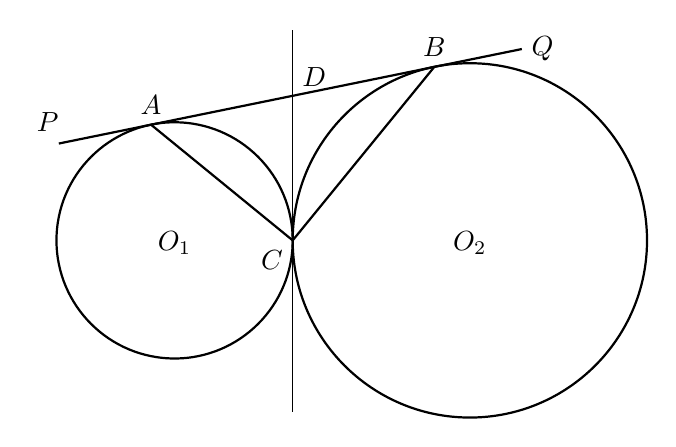
\begin{tikzpicture}[scale=1.5]
  \draw[thick] (0,0) circle (1);
  \draw[thick] (2.5,0) circle (1.5);
  \draw[thick] (-0.98,0.82)--(2.94,1.62);
  \draw[thin] (1,1.78)--(1,-1.45);
  \draw[thick] (-0.2,0.98)--(1,0);
  \draw[thick] (2.2,1.47)--(1,0);
  \node[above left] at (-0.9,0.84) {$P$};
  \node[above] at (-0.2,0.98) {$A$};
  \node[above right] at (1,1.22) {$D$};
  \node[above] at (2.2,1.47) {$B$};
  \node[right] at (2.94,1.62) {$Q$};
  \node at (0,-0.02) {$O_1$};
  \node at (2.5,-0.02) {$O_2$};
  \node[below left] at (1,0) {$C$};
\end{tikzpicture}
\end{center}
\nopagebreak[4]
\Needspace{4\baselineskip}
\textbf{解析}
\nopagebreak[4]
\begin{center}% 1977 年云南卷第 3 题：两圆 O1、O2 外切于 C，外公切线 PQ 切两圆于 A、B，
% 过 C 的内公切线交 PQ 于 D，连接 AC、BC（按源卷第 2 页布局）
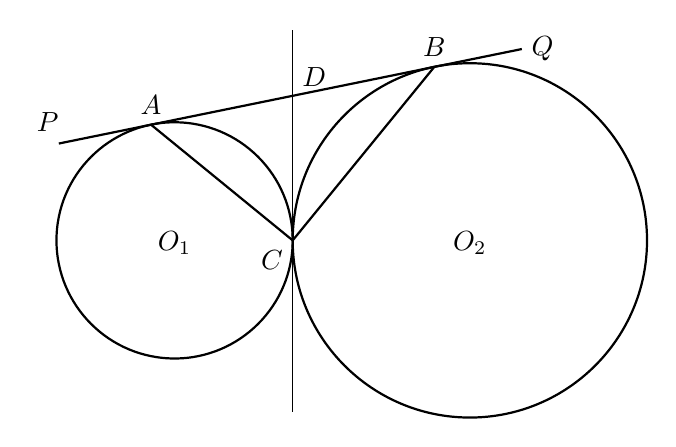
\begin{tikzpicture}[scale=1.5]
  \draw[thick] (0,0) circle (1);
  \draw[thick] (2.5,0) circle (1.5);
  \draw[thick] (-0.98,0.82)--(2.94,1.62);
  \draw[thin] (1,1.78)--(1,-1.45);
  \draw[thick] (-0.2,0.98)--(1,0);
  \draw[thick] (2.2,1.47)--(1,0);
  \node[above left] at (-0.9,0.84) {$P$};
  \node[above] at (-0.2,0.98) {$A$};
  \node[above right] at (1,1.22) {$D$};
  \node[above] at (2.2,1.47) {$B$};
  \node[right] at (2.94,1.62) {$Q$};
  \node at (0,-0.02) {$O_1$};
  \node at (2.5,-0.02) {$O_2$};
  \node[below left] at (1,0) {$C$};
\end{tikzpicture}
\end{center}
\nopagebreak[4]
\Needspace{5\baselineskip}
过 $C$ 作两园的内公切线，与 $PQ$ 交于 $D$。由切线长定理，

\nopagebreak[4]
\[
DA=DC,\qquad DB=DC,
\]

\Needspace{5\baselineskip}
从而

\nopagebreak[4]
\[
\angle DAC=\angle DCA,\qquad
\angle DCB=\angle DBC.
\]

\Needspace{5\baselineskip}
$A$、$D$、$B$ 同在切线 $PQ$ 上，故

\nopagebreak[4]
\[
\angle DAC+\angle DCA+\angle DCB+\angle DBC=180^\circ,
\]

\Needspace{5\baselineskip}
代入两组等角得

\nopagebreak[4]
\[
2(\angle DCA+\angle DCB)=180^\circ
\quad\Longrightarrow\quad
\angle ACB=\angle DCA+\angle DCB=90^\circ,
\]

即 $AC\perp BC$。

\gkanswer{答案：见解析版}

\end{answer}
\begin{answer}
\gksolhead{4}{}

\textbf{题目}：

求过 $x^2+y^2=4$ 上一点 $P(1,\sqrt3)$ 的切线 $L$ 的方程。

\Needspace{4\baselineskip}
\textbf{解析}

\Needspace{5\baselineskip}
圆 $x^2+y^2=4$ 的圆心为原点、半径为 $2$，且 $1+3=4$，点 $P(1,\sqrt3)$ 在圆上。半径 $OP$ 的斜率为 $\sqrt3$，切线与半径垂直，斜率为 $-\dfrac1{\sqrt3}$：

\nopagebreak[4]
\[
y-\sqrt3=-\frac1{\sqrt3}(x-1)
\quad\Longrightarrow\quad
x+\sqrt3\,y-4=0.
\]

\gkanswer{答案：$x+\sqrt3\,y-4=0$。}

\end{answer}
\begin{answer}
\gksolhead{5}{}

\textbf{题目}（15 分）：

一船以 24 浬/小时的速度向正北航行，在 $A_1$ 点望见一灯塔 $S$，在船的北偏东 $30^\circ$，15 分钟后，在 $A_2$ 点望见灯塔在船的北偏东 $65^\circ$（如图），求船在 $A_2$ 点时与灯塔的距离 $A_2S$。（已知 $\sin35^\circ=0.574$）

\begin{gktip}
原源 PDF 第 3 页附有航向与灯塔方位示意图；LaTeX 版按源图重绘。
\end{gktip}
\nopagebreak[4]
\begin{center}% 1977 年云南卷第 5 题：船沿正北航道自 A1 行至 A2，灯塔 S 在 A1 的北偏东 30°、
% 在 A2 的北偏东 65°，北向箭头标「北」（按源卷第 3 页布局）
\begin{tikzpicture}[scale=1.6]
  \draw[->,thick] (0,-0.35)--(0,3.3);
  \draw[thick] (0,0)--(1.58,2.74);
  \draw[thick] (0,2)--(1.58,2.74);
  \node[above] at (0,3.3) {北};
  \node[above right] at (1.58,2.74) {$S$};
  \node[left] at (0,2) {$A_2$};
  \node[below] at (0,0) {$A_1$};
  \node at (0.42,2.60) {$65^\circ$};
  \node at (0.26,0.85) {$30^\circ$};
\end{tikzpicture}
\end{center}
\nopagebreak[4]
\Needspace{4\baselineskip}
\textbf{解析}
\nopagebreak[4]
\begin{center}% 1977 年云南卷第 5 题：船沿正北航道自 A1 行至 A2，灯塔 S 在 A1 的北偏东 30°、
% 在 A2 的北偏东 65°，北向箭头标「北」（按源卷第 3 页布局）
\begin{tikzpicture}[scale=1.6]
  \draw[->,thick] (0,-0.35)--(0,3.3);
  \draw[thick] (0,0)--(1.58,2.74);
  \draw[thick] (0,2)--(1.58,2.74);
  \node[above] at (0,3.3) {北};
  \node[above right] at (1.58,2.74) {$S$};
  \node[left] at (0,2) {$A_2$};
  \node[below] at (0,0) {$A_1$};
  \node at (0.42,2.60) {$65^\circ$};
  \node at (0.26,0.85) {$30^\circ$};
\end{tikzpicture}
\end{center}
\nopagebreak[4]
\Needspace{5\baselineskip}
船 15 分钟航行

\nopagebreak[4]
\[
A_1A_2=24\times\frac{15}{60}=6\ \text{（\text{浬}）}.
\]

\Needspace{5\baselineskip}
在 $\triangle A_1A_2S$ 中，$\angle A_2A_1S=30^\circ$，$\angle A_1A_2S=180^\circ-65^\circ=115^\circ$，于是

\nopagebreak[4]
\[
\angle A_1SA_2=180^\circ-30^\circ-115^\circ=35^\circ
\quad(=65^\circ-30^\circ).
\]

\Needspace{5\baselineskip}
由正弦定理，

\nopagebreak[4]
\[
\frac{A_2S}{\sin30^\circ}=\frac{A_1A_2}{\sin35^\circ},
\qquad
A_2S=\frac{6\sin30^\circ}{\sin35^\circ}
=\frac{6\times\dfrac12}{0.574}
\approx5.23\ \text{（\text{浬}）}.
\]

\gkanswer{答案：$A_2S=\dfrac{6\sin30^\circ}{\sin35^\circ}\approx5.23$ 浬。}

\end{answer}
\begin{answer}
\gksolhead{6}{}

\textbf{题目}：

直角三角形中的一个锐角为 $\beta$，面积是 12。

（1） 求此三角形的外接园的面积；

（2） 当 $\beta$ 取何值时，外接园的面积最小。

\begin{gktip}
原源 PDF 第 3 页附有直角三角形及其外接园示意图；LaTeX 版按源图重绘。
\end{gktip}
\nopagebreak[4]
\begin{center}% 1977 年云南卷第 6 题：直角三角形 ABC 内接于外接圆，斜边 AB 为直径 2R，
% 直角在 C（带直角标记），锐角 β 在 B 处（按源卷第 3 页布局）
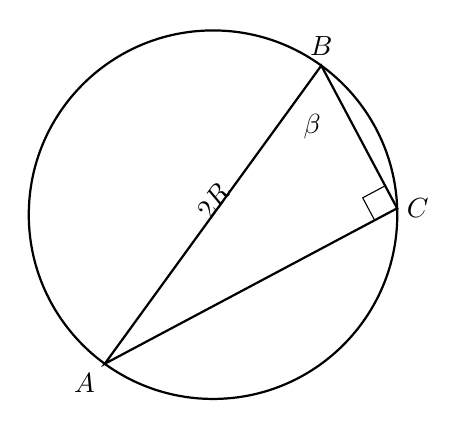
\begin{tikzpicture}[scale=1.8]
  \draw[thick] (0,0) circle (1.3);
  \draw[thick] (-0.764,-1.052)--(0.764,1.052)--(1.299,0.045)--cycle;
  \draw[thin] (1.140,-0.039)--(1.056,0.119)--(1.215,0.204);
  \node[below left] at (-0.764,-1.052) {$A$};
  \node[above] at (0.764,1.052) {$B$};
  \node[right] at (1.299,0.045) {$C$};
  \node[rotate=54] at (0,0.10) {$2R$};
  \node at (0.70,0.62) {$\beta$};
\end{tikzpicture}
\end{center}
\nopagebreak[4]
\Needspace{4\baselineskip}
\textbf{解析}

\Needspace{5\baselineskip}
设外接园半径为 $R$。直角三角形的斜边即外接园的直径 $2R$，设 $\angle B=\beta$，则两条直角边分别为

\nopagebreak[4]
\[
2R\sin\beta
\qquad\text{\text{和}}\qquad
2R\cos\beta.
\]

\Needspace{5\baselineskip}
由面积条件，

\nopagebreak[4]
\[
\frac12\cdot2R\sin\beta\cdot2R\cos\beta
=R^{2}\sin2\beta=12,
\qquad
R^{2}=\frac{12}{\sin2\beta}.
\]

\gksubpart{（1）}

\Needspace{5\baselineskip}
外接园面积

\nopagebreak[4]
\[
\pi R^{2}=\frac{12\pi}{\sin2\beta}.
\]

\gksubpart{（2）}

$\beta$ 为锐角，$0<2\beta<180^\circ$，$\sin2\beta\le1$，故 $\pi R^{2}\ge12\pi$；当 $\sin2\beta=1$，即 $\beta=45^\circ$ 时外接园面积最小，最小值为 $12\pi$。
\nopagebreak[4]
\begin{center}% 1977 年云南卷第 6 题：直角三角形 ABC 内接于外接圆，斜边 AB 为直径 2R，
% 直角在 C（带直角标记），锐角 β 在 B 处（按源卷第 3 页布局）
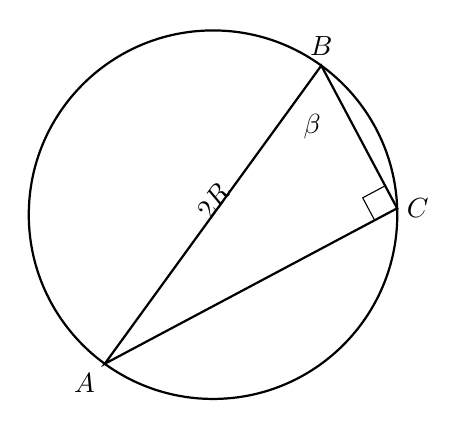
\begin{tikzpicture}[scale=1.8]
  \draw[thick] (0,0) circle (1.3);
  \draw[thick] (-0.764,-1.052)--(0.764,1.052)--(1.299,0.045)--cycle;
  \draw[thin] (1.140,-0.039)--(1.056,0.119)--(1.215,0.204);
  \node[below left] at (-0.764,-1.052) {$A$};
  \node[above] at (0.764,1.052) {$B$};
  \node[right] at (1.299,0.045) {$C$};
  \node[rotate=54] at (0,0.10) {$2R$};
  \node at (0.70,0.62) {$\beta$};
\end{tikzpicture}
\end{center}
\nopagebreak[4]
\gkanswer{答案（1）：$\dfrac{12\pi}{\sin2\beta}$。}

\gkanswer{答案（2）：当 $\beta=45^\circ$ 时外接园面积最小，最小值为 $12\pi$。}

\end{answer}
\begin{answer}
\gksolhead{7}{}

\textbf{题目}（15 分）：

一个三角形三边的比为 $4:5:6$，面积为 $27\sqrt7\ \mathrm{cm^2}$，求三边之长。

\textbf{参考题 1．} 某生产队要建造一个体积为 50 立方米的有盖园柱形氨水池（如图），问这个氨水池高和底半径取多大时用料最省（即表面积最小）？

\begin{gktip}
原源 PDF 第 4 页附有有盖园柱形氨水池示意图；LaTeX 版按源图重绘。
\end{gktip}
\nopagebreak[4]
\begin{center}% 1977 年云南卷参考题 1：有盖圆柱形氨水池示意图，虚线轴上标高 h，
% 顶面自圆心画一段半径（按源卷第 4 页布局）
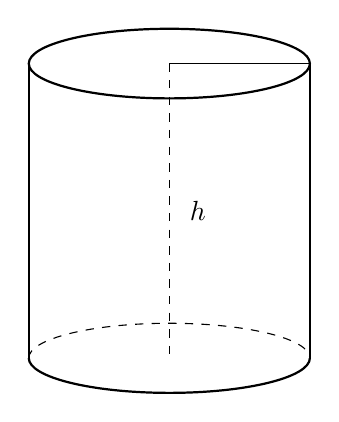
\begin{tikzpicture}[scale=1.7]
  \draw[thick] (0,2.2) ellipse (1.05 and 0.26);
  \draw[thick] (-1.05,0)--(-1.05,2.2);
  \draw[thick] (1.05,0)--(1.05,2.2);
  \draw[thick] (-1.05,0) arc (180:360:1.05 and 0.26);
  \draw[dashed] (-1.05,0) arc (180:0:1.05 and 0.26);
  \draw[thin] (0,2.2)--(1.05,2.2);
  \draw[dashed] (0,2.2)--(0,0);
  \node[right] at (0.08,1.1) {$h$};
\end{tikzpicture}
\end{center}
\nopagebreak[4]
\Needspace{5\baselineskip}
\textbf{参考题 2．} 求

\nopagebreak[4]
\[
\int_0^2\frac{x}{\sqrt{1+x^2}}\,dx.
\]

\Needspace{4\baselineskip}
\textbf{解析}

\Needspace{5\baselineskip}
设三边为 $a=4x$、$b=5x$、$c=6x$（单位 cm），半周长

\nopagebreak[4]
\[
s=\frac{4x+5x+6x}{2}=\frac{15}{2}x,
\]

\nopagebreak[4]
\[
s-a=\frac{7}{2}x,\qquad
s-b=\frac{5}{2}x,\qquad
s-c=\frac{3}{2}x.
\]

\Needspace{5\baselineskip}
由海伦公式，

\nopagebreak[4]
\[
\sqrt{s(s-a)(s-b)(s-c)}
=\sqrt{\frac{15x}{2}\cdot\frac{7x}{2}\cdot\frac{5x}{2}\cdot\frac{3x}{2}}
=\frac{15\sqrt7}{4}x^{2}.
\]

\Needspace{5\baselineskip}
令其等于 $27\sqrt7$：

\nopagebreak[4]
\[
\frac{15\sqrt7}{4}x^{2}=27\sqrt7
\quad\Longrightarrow\quad
x^{2}=\frac{36}{5},
\qquad
x=\frac{6\sqrt5}{5}.
\]

\Needspace{5\baselineskip}
所以

\nopagebreak[4]
\[
a=\frac{24}{5}\sqrt5,\qquad
b=6\sqrt5,\qquad
c=\frac{36}{5}\sqrt5
\quad\text{（cm）}.
\]

\textbf{参考题 1}

\Needspace{5\baselineskip}
设底半径 $r$ 米、高 $h$ 米。体积条件

\nopagebreak[4]
\[
\pi r^{2}h=50
\quad\Longrightarrow\quad
h=\frac{50}{\pi r^{2}}.
\]

\Needspace{5\baselineskip}
有盖表面积

\nopagebreak[4]
\[
S=2\pi r^{2}+2\pi rh
=2\pi r^{2}+\frac{100}{r}.
\]

\Needspace{5\baselineskip}
\textbf{解法一（导数）}：

\nopagebreak[4]
\[
S'=4\pi r-\frac{100}{r^{2}},
\qquad
S''=4\pi+\frac{200}{r^{3}}>0\quad(r>0).
\]

\Needspace{5\baselineskip}
令 $S'=0$ 得 $r^{3}=\dfrac{25}{\pi}$，即 $r=\sqrt[3]{\dfrac{25}{\pi}}$，此时

\nopagebreak[4]
\[
h=\frac{50}{\pi r^{2}}=2\sqrt[3]{\frac{25}{\pi}}=2r,
\]

$S$ 取最小值。即高等于底面直径时用料最省。

\Needspace{5\baselineskip}
\textbf{解法二（均值不等式）}：

\nopagebreak[4]
\[
S=2\pi r^{2}+\frac{50}{r}+\frac{50}{r}
\ge3\sqrt[3]{2\pi r^{2}\cdot\frac{50}{r}\cdot\frac{50}{r}}
=3\sqrt[3]{5000\pi}\quad\text{（\text{常数}）},
\]

当 $2\pi r^{2}=\dfrac{50}{r}$，即 $r=\sqrt[3]{\dfrac{25}{\pi}}$ 时取等号，结论相同。

\textbf{参考题 2}

\Needspace{5\baselineskip}
因 $\left(\sqrt{1+x^{2}}\right)'=\dfrac{x}{\sqrt{1+x^{2}}}$，故

\nopagebreak[4]
\[
\int_0^2\frac{x}{\sqrt{1+x^{2}}}\,dx
=\sqrt{1+x^{2}}\ \Big|_0^2
=\sqrt5-1.
\]

\gkanswer{答案：三边之长分别为 $\dfrac{24}{5}\sqrt5\ \mathrm{cm}$、$6\sqrt5\ \mathrm{cm}$、$\dfrac{36}{5}\sqrt5\ \mathrm{cm}$。}

\end{answer}